% !TeX root = ../main.tex
% Add the above to each chapter to make compiling the PDF easier in some editors.

\chapter{Union-Find with Explain Operation}\label{chapter:union_find}

\section{Union-Find Algorithm}
\label{section:uf-algorithm}

Given a set of $n$ elements, the union-find data structure keeps track of a partition of these elements in disjoint sets. It provides efficient operations for finding the set that an element belongs in and for modifying the sets.

In the beginning, each element is in its own set, then the sets are merged by subsequent \emph{union} operations between pairs of elements. Each set in the partition has a representative, which is one particular element in the set. We will denote the representative of an element $a$ in the union-find forest $l$ as $rep\_of(l, a)$. The \emph{find} operation returns the representative of the set that a certain element belongs to. If two elements have the same representative, that means that they belong to the same set. The elements of the union-find data structure are represented by the natural numbers $0,1,...,n-1$.

One application of this algorithm is to maintain the equivalence closure of equations. Given a set of $n$ variables, we can initialize the union-find algorithm with $n$ elements, and for each equation $a_1 = a_2$ we perform a \emph{union} between $a_1$ and $a_2$. Each set in the partition represents an equivalence class.

The equivalence classes are modeled with a forest, which is a graph where each connected component is a tree. The connected components of the graph represent the equivalence classes. Initially, the graph contains $n$ vertices and no edges, then each \lstinline{union} adds a directed edge.  Each tree in the forest has a root, which is also the representative of the equivalence class, and each edge in the tree is directed towards the root. In order to keep this invariant, at each \emph{union} between $a$ and $b$, the new edge is added between the $rep\_of(l,a)$ and $rep\_of(l, b)$.

The union-find forest is represented by a list $l$ of length $n$, where at each index $i$ the list contains the parent of the element $i$ in the forest.
Mimicking the Isabelle syntax for lists, we will denote the representative of an element $a$ as $l ! a$.
If $i$ does not have a parent, then the list contains the element $i$ itself at the index $i$, i.e., $l!i = i$. This means that $i$ is a root.

The original union-find algorithm \cite{Tarjan} contains two optimizations: the first one adds a direct edge from each visited node to its representative in the \emph{find} method (path compression). The second one chooses the representative of the larger class to be the new representative of the merged class in \emph{union} (union by rank). These optimizations are irrelevant for the correctness of the algorithm, therefore we leave them out of this implementation in order to simplify the proofs.

Most of the proofs about the following algorithms contains as an assumption that all variables are in bound, i.e. $x < n$ for each variable $x$.
More precisely, the parameter $n$ is characterized by the length of the list $l$, therefore the assumption is $x < length(l)$.
For reasons of conciseness, assumptions of this kind will not be mentioned in the thesis. The same applies to the theorems about congruence closure in the next chapter.
For the exact formulation of the lemmas, refer to the Isabelle code.

\section{Union-Find in Isabelle/HOL}
\label{section:uf-isabelle}

The union-find algorithm was already formalized in Isabelle/HOL by Lammich \cite{unionfind-isabelle}, and the code can be found in the ``Archive of Formal Proofs'' (AFP) under ``A Separation Logic Framework for Imperative HOL'', in the theory ``Union\_Find''\cite{afp, Sep}. The following is a brief description of the implementation.

The function \lstinline{rep_of} finds the representative of an element in the forest. It is analogous to the \lstinline{find} operation, except that it does not do path compression.

\begin{lstlisting}
function (domintros) rep_of
  where "rep_of l i = (if l!i = i then i else rep_of l (l!i))"
  by pat_completeness auto
\end{lstlisting}

The domain of \lstinline{rep_of} is used to define the following invariant for valid union-find lists. This invariant states that the \lstinline{rep_of} function terminates on all valid indexes of the list, which is equivalent to affirming that the union-find forest does not contain any cycles.

\begin{lstlisting}
definition "ufa_invar l ≡ ∀i<length l. rep_of_dom (l,i) ∧ l!i<length l"
\end{lstlisting}

The \lstinline{union} operation simply adds an edge between the representatives of the two elements.

\begin{lstlisting}
abbreviation "ufa_union l x y ≡ l[rep_of l x := rep_of l y]"
\end{lstlisting}

The theory contains several lemmas, including a lemma which states that the invariant \lstinline{ufa_invar} holds for the initial union-find forest without edges, and that it is preserved by the \lstinline{ufa_union} operation.

\section{Union-Find Data Structure}
\label{section:uf-data}

The section below describes the implementation of a union-find data structure.
It contains the union-find forest described in Section \ref{section:uf-algorithm}, as well as two other lists that are useful for the implementation of the \emph{explain} operation. They are described in the following. For a more detailed explanation refer to \cite{Nieuwenhuis}.

\begin{itemize}
	\item \lstinline{uf_list}: This is the usual union-find list, which contains the parent node of each element in the forest data structure. It is the one described in Section \ref{section:uf-algorithm}.

	\item \lstinline{unions}: This list simply contains all the pairs of input elements in chronological order.

	\item \lstinline{au}: This is the \emph{associated unions} list, it contains for each edge in the union-find forest a label with the union that is associated to this edge. Each \emph{union} adds exactly one edge to the forest and when it is added, we also label this edge with the arguments of the \emph{union}. Similarly to the \lstinline{uf_list}, \lstinline|au| is indexed by the element. For each element $b$ which is not a root, \lstinline{au} contains the input equation which caused the creation of this edge between $b$ and its parent. The equations are represented as indexes into the \lstinline{unions} list. The type of the entries is \lstinline{nat option}, so that for elements which are roots, the \lstinline{au} entry is \lstinline{None}.
\end{itemize}

\begin{exmp}\label{empty_ufe}
For a union-find algorithm with 4 variables, the initial empty data structure looks as follows:
\begin{lstlisting}
⦇uf_list = [0, 1, 2, 3], unions = [], au = [None, None, None, None]⦈
\end{lstlisting}
Each element is its own parent in the \lstinline{uf_list}, which means that it is a root. The \lstinline{unions} list is empty because no unions were made yet.
There are no edges in the tree, therefore there are no labels in \lstinline{au}.
\end{exmp}

In order to implement the \emph{explain} operation, we need functions that find the path between two nodes and the lowest common ancestor of two elements.
In order to reason about paths and formalize the correctness theorems of these functions, we define the following abstraction of paths.

\begin{lstlisting}
inductive path :: "nat list ⇒ nat ⇒ nat list ⇒ nat ⇒ bool" where
  single: "n < length l ⟹ path l n [n] n" |
  step: "r < length l ⟹ l ! u = r ⟹ l ! u ≠ u ⟹  path l u p v ⟹ path l r (r # p) v"
\end{lstlisting}

A path from $r$ to $v$ is written as \lstinline{path l r p v}. The node $r$ is an ancestor of $v$, hence it is closer to the root. $p$ is a list which contains all the nodes visited on the path from $r$ to $v$. This definition proved to be very useful for several proofs, as will become clearer in the following sections.

The theory ``Path'' contains various lemmas about paths, including lemmas about concatenation of paths.
For a complete overview of the proofs, refer to the Isabelle code.
Most theorems about paths could be proven by rule induction on \lstinline{path}.
The most interesting and useful lemma is about the uniqueness of paths between two nodes. The proof uses the fact that the union-find forest does not have cycles if \lstinline|ufa_invar| holds.

\begin{lstlisting}
theorem path_unique: "ufa_invar l ⟹ path l u p1 v ⟹ path l u p2 v ⟹ p1 = p2"
\end{lstlisting}


\section{Implementation}

\subsection{Union}

The \lstinline{ufa_union} operation needs to be extended in order to appropiately update the other two lists, therefore we introduce the function \lstinline{ufe_union}. The \lstinline|"e"| in the name of the function indicates that it was implemented in order to support an \emph{explain} function.

The function \lstinline{ufe_union} only modifies the data structure if the parameters are not already in the same equivalence class.
The \lstinline{uf_list} is modified with \lstinline{ufa_union}.
The current union $(x, y)$ is appended to the end of the \lstinline{unions} list.
\lstinline{au} is updated such that the new edge between \lstinline{rep_of l x} and \lstinline{rep_of l y} is labeled with the last index of \lstinline{unions}, which contains the current pair of elements $(x, y)$.

\begin{lstlisting}
fun ufe_union :: "ufe_data_structure ⇒ nat ⇒ nat ⇒ ufe_data_structure"
  where
    "ufe_union ⦇uf_list = l, unions = u, au = a⦈ x y = (
if (rep_of l x ≠ rep_of l y) then
    ⦇uf_list = ufa_union l x y,
     unions = u @ [(x,y)],
     au = a[rep_of l x := Some (length u)]⦈
else ⦇uf_list = l, unions = u, au = a⦈)"
\end{lstlisting}

\begin{exmp}
After a union of 3 and 2, the data structure from Example \ref{empty_ufe} looks as follows:
\begin{lstlisting}
⦇uf_list= [0, 1, 2, 2], unions = [(3, 2)], au = [None, None, None, Some 0]⦈
\end{lstlisting}
It has the following graphical representation:
\begin{center}
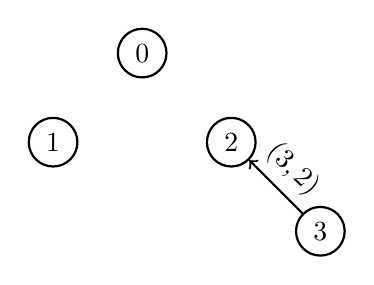
\begin{tikzpicture}[node distance={16mm}, thick, main/.style = {draw, circle}]
\node[main] (0) {0};
\node[main] (1) [below left of=0] {1};
\node[main] (2) [below right of=0] {2};
\node[main] (3) [below right of=2] {3};
\draw[->] (3) -- node[midway, above, sloped]{$(3,2)$} (2);
\end{tikzpicture}
\end{center}

\end{exmp}

In Subsection \ref{subsection:invariant}, we will define an invariant that characterizes well-formed union-find data structures.
The invariant states that the data structure can be generated by subsequently applying \lstinline|ufe_union|.
In order to define this invariant, we first introduce a function which takes a list of unions as parameter and simply applies each of those unions to the data structure.

\begin{lstlisting}
fun apply_unions :: "(nat * nat) list ⇒ ufe_data_structure ⇒ ufe_data_structure"
  where
    "apply_unions [] p = p" |
    "apply_unions ((x, y) # u) p = apply_unions u (ufe_union p x y)"
\end{lstlisting}

\begin{exmp}\label{example:apply-unions}
Let \lstinline|initial_ufe n| be the empty union-find list with $n$ variables. The result of \lstinline|apply_unions [(3,2), (3,0), (1,0)] (initial_ufe 4)| is the following:

\begin{center}
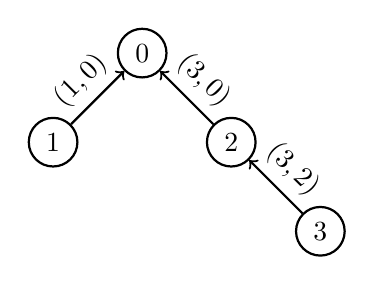
\begin{tikzpicture}[node distance={16mm}, thick, main/.style = {draw, circle}]
\node[main] (0) {0};
\node[main] (1) [below left of=0] {1};
\node[main] (2) [below right of=0] {2};
\node[main] (3) [below right of=2] {3};
\draw[->] (3) -- node[midway, above, sloped]{$(3,2)$} (2);
\draw[->] (2) -- node[midway, above, sloped]{$(3,0)$} (0);
\draw[->] (1) -- node[midway, above, sloped]{$(1,0)$} (0);
\end{tikzpicture}
\end{center}
\end{exmp}

\subsection{Helper Functions for Explain}\label{subsection:helper-functions}

We implement the \lstinline|explain| function following the description of the first version of the union-find algorithm in the paper by Nieuwenhuis et al. \cite{Nieuwenhuis}

The \lstinline|explain| function takes as parameters two elements $x$ and $y$ and calculates a subset of the input unions which explain why the two given variables are in the same equivalence class. The input unions are the ones present in the \lstinline|unions| list. If we consider the graph which has as nodes the constants and as edges the input unions, then the output of \lstinline|explain| would be all the unions on the path from $x$ to $y$. However, the union-find forest in our data structure is different than the aforementioned graph. It does not have as edges the unions, because \lstinline|ufa_union l x y| adds an edge between $rep\_of(l, x)$ and $rep\_of(l, y)$, instead of an edge between $x$ and $y$.

Let $(a, b)$ be the last union made between the equivalence class of $x$ and the one of $y$.
The last union corresponds to the maximal label in \lstinline|au|, because the labels in \lstinline|au| are indexes into the \lstinline|unions| list and the equations in \lstinline|unions| are in chronological order.
An example of the structure of the union-find forest is given by the following visualization:

\begin{center}
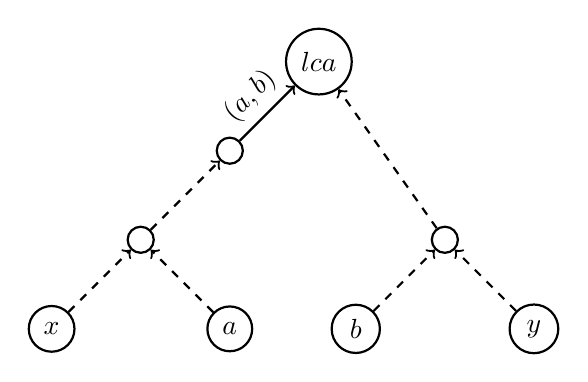
\begin{tikzpicture}[node distance={16mm}, thick, main/.style = {draw, circle}]
\node[main] (x) {$x$};
\node[main] (f1) [above right of=x] {};
\node[main] (a) [below right of=f1] {$a$};
\node[main] (b) [right of=a] {$b$};
\node[main] (f3) [above right of=b] {};
\node[main] (y) [below right of=f3] {$y$};
\node[main] (f2) [above right of=f1] {};
\node[main] (lca) [above right of=f2] {$lca$};
\draw[->] (f2) -- node[midway, above, sloped]{$(a,b)$} (lca);
\draw[->, dashed] (x) -- (f1);
\draw[->, dashed] (f1) -- (f2);
\draw[->, dashed] (a) -- (f1);
\draw[->, dashed] (b) -- (f3);
\draw[->, dashed] (f3)-- (lca);
\draw[->, dashed] (y) -- (f3);
\end{tikzpicture}
\end{center}

We can calculate the desired output of \lstinline|explain| by first adding  $(a, b)$ to the output and then recursively calling the \lstinline|explain| operation with the new parameters $(x, a)$ and $(b, y)$ (or $(x, b)$ and $(a, y)$, depending on which branch $a$ and $b$ are on).

The pair $(a, b)$ is calculated by finding the lowest common ancestor $lca$ of $x$ and $y$, and then finding the newest union on the paths from $x$ to $lca$ and from $y$ to $lca$.

This section describes the helper functions needed for the implementation of \lstinline|explain|, which calculate the lowest common ancestor, using the function \lstinline{path_to_root}, and the newest union on a path.

\subsubsection{path\_to\_root}
\label{subsubsection:path-to-root}

The function \lstinline{path_to_root l x} computes the path from $rep\_of(l,x)$ to the node $x$ in the union-find forest $l$. It simply starts at $x$ and continues to add the parent of the current node to the front of the path, until it reaches the root.

\begin{lstlisting}
function path_to_root :: "nat list ⇒ nat ⇒ nat list"
  where
    "path_to_root l x =
        (if l ! x = x then [x]
            else path_to_root l (l ! x) @ [x])"
  by pat_completeness auto
\end{lstlisting}

\begin{exmp}
If we consider $l$ to be the union-find list of Example \ref{example:apply-unions}, then

\lstinline|path_to_root l 3 = [0, 2, 3]|.
\end{exmp}

It was straightforward to show that it has the same domain as the \lstinline{rep_of} function, as it has the same recursive calls.

\begin{lstlisting}
lemma path_to_root_domain: "rep_of_dom (l, i) ⟷ path_to_root_dom (l, i)"
\end{lstlisting}

The correctness of the function follows directly by computation induction.

\begin{lstlisting}
theorem path_to_root_correct:
  assumes "ufa_invar l"
  shows "path l (rep_of l x) (path_to_root l x) x"
\end{lstlisting}

\subsubsection{lowest\_common\_ancestor}

The function \lstinline{lowest_common_ancestor l x y} finds the lowest common ancestor of $x$ and $y$ in the union-find forest $l$.
A \emph{common ancestor} of two nodes $x$ and $y$ is a node which has a path to $x$ and a path to $y$.
The \emph{lowest common ancestor} of two nodes $x$ and $y$ is the common ancestor which is farthest away from the root.

The function will only be used for two nodes which have the same root, otherwise there is no common ancestor. It first computes the paths from $x$ and $y$ to their root, and then returns the last element which the two paths have in common. For this it uses the function \lstinline{longest_common_prefix} from ``HOL-Library.Sublist'', which is included in the standard Isabelle distribution.

\begin{lstlisting}
fun lowest_common_ancestor :: "nat list ⇒ nat ⇒ nat ⇒ nat"
  where
    "lowest_common_ancestor l x y =
last (longest_common_prefix (path_to_root l x) (path_to_root l y))"
\end{lstlisting}

\begin{exmp}
If we consider $l$ to be the union-find list of Example \ref{example:apply-unions}, then

\lstinline|lowest_common_ancestor l 3 1 = 0|.
\end{exmp}

Regarding the correctness proof, there are two aspects to prove: the most useful result is that \lstinline{lowest_common_ancestor l x y} is a common ancestor of $x$ and $y$. The second aspect states that any other common ancestor of $x$ and $y$ has a shorter distance from the root. The proof assumes that $x$ and $y$ have the same root.

First, we define that a common ancestor of $x$ and $y$ is a node $ca$ that has a path to $x$ and a path to $y$.

\begin{lstlisting}
abbreviation "common_ancestor l x y ca ≡
(∃ p . path l ca p x) ∧
(∃ p . path l ca p y)"
\end{lstlisting}

The lowest common ancestor $lca$ is a common ancestor where each other common ancestor has a shorter distance from the root $r$.

\begin{lstlisting}
abbreviation "is_lca l x y lca ≡
(common_ancestor l x y lca ∧
(∀r ca$_2$ p$_1$ p$_2$. path l r p$_1$ lca ∧ path l r p$_2$ ca$_2$ ∧ common_ancestor l x y ca$_2$
⟶ length p$_1$ ≥ length p$_2$))"
\end{lstlisting}

Now we can define the correctness theorem.

\begin{lstlisting}
theorem lowest_common_ancestor_correct:
  assumes "ufa_invar l"
    and "rep_of l x = rep_of l y"
  shows "is_lca l x y (lowest_common_ancestor l x y)"
\end{lstlisting}

\begin{proof}
Let $lca =$\lstinline{lowest_common_ancestor l x y}. We previously proved that \lstinline{path_to_root} computes a path $p_x$ from the root to $x$ and a path $p_y$ from the root to $y$. Evidently, $lca$ lies on both paths, because it is part of their common prefix. Splitting the path $p_x$, we get a path from the root to $lca$ and one from $lca$ to $x$, and the same for $y$. This shows that $lca$ is a common ancestor.

To prove that it is the \emph{lowest} common ancestor, we can prove it by contradiction. We assume that there is a common ancestor $lca_2$ with a longer path from the root than $lca$. We show that there is a path from the root to $x$ passing through $lca_2$, and the same for $y$. Because of the uniqueness of paths, these paths are equal to \lstinline{path_to_root l x} and \lstinline{path_to_root l y}, respectively. That means, that there is a prefix of \lstinline{path_to_root l x} and \lstinline{path_to_root l y} which is longer than the one calculated by the function \lstinline{longest_common_prefix}. The theory ``Sublist'' contains a correctness proof for \lstinline{longest_common_prefix}, which we can use to show the contradiction.
\end{proof}

\subsubsection{find\_newest\_on\_path}

The function \lstinline{find_newest_on_path l a x y} finds the newest edge on the path from $y$ to $x$. It is assumed that $y$ is an ancestor of $x$. The function simply scans all the elements on the path from $y$ to $x$ and returns the one with the largest index in $a$, the \emph{associated unions} list.

\begin{lstlisting}
function (domintros) find_newest_on_path  :: "nat list ⇒ nat option list ⇒ nat ⇒ nat ⇒ nat option"
  where
    "find_newest_on_path l a x y =
  (if x = y then None
    else max (a ! x) (find_newest_on_path l a (l ! x) y))"
  by pat_completeness auto
\end{lstlisting}

\begin{exmp}
Let $l$ be the union-find list of Example \ref{example:apply-unions}. If we consider the edge labels in the associated unions list instead of the unions they represent, the union-find graph looks like this:

\begin{center}
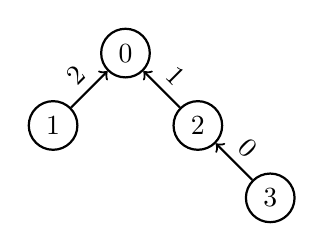
\begin{tikzpicture}[node distance={13mm}, thick, main/.style = {draw, circle}]
\node[main] (0) {0};
\node[main] (1) [below left of=0] {1};
\node[main] (2) [below right of=0] {2};
\node[main] (3) [below right of=2] {3};
\draw[->] (3) -- node[midway, above, sloped]{0} (2);
\draw[->] (2) -- node[midway, above, sloped]{1} (0);
\draw[->] (1) -- node[midway, above, sloped]{2} (0);
\end{tikzpicture}
\end{center}

From this representation we can see that the newest label on the path from 3 to 0 is 1 and on the path from 1 to 0 it is 2.
\end{exmp}

If there is a path $p$ from $y$ to $x$, it is easily shown by induction that the function terminates.

\begin{lstlisting}
lemma find_newest_on_path_domain:
  assumes "ufa_invar l"
    and "path l y p x"
  shows "find_newest_on_path_dom (l, a, x, y)"
\end{lstlisting}

For the correctness proof, we define an abstract definition of the newest element on the path: \lstinline{Newest_on_path} is the maximal value in the \emph{associated unions} list for indexes in $p$.

\begin{lstlisting}
abbreviation "Newest_on_path l a x y newest ≡
∃ p . path l y p x ∧ newest = (MAX i ∈ set [1..<length p]. a ! (p ! i))"
\end{lstlisting}

Then it can easily be shown by computation induction on \lstinline{find_newest_on_path} that the function is correct.

\begin{lstlisting}
theorem find_newest_on_path_correct:
  assumes "path l y p x"
    and "ufa_invar l"
    and "x ≠ y"
  shows "Newest_on_path l a x y (find_newest_on_path l a x y)"
\end{lstlisting}

\subsection{Explain}

We define the \lstinline|explain| operation, as described in Subsection \ref{subsection:helper-functions}.
If $rep\_of(l, x) \neq rep\_of(l, y)$, then $x$ and $y$ are not be in the same equivalence class and we cannot produce an explanation.
The function terminates when $x = y$.
Otherwise, the lowest common ancestor between $x$ and $y$ is determined.
Next, we first compute the newest edge on the $x$ branch, then the one on the $y$ branch, and afterwards we make a case distinction to choose the larger one.

\begin{exmp}
Let $ufe$ be the union-find data structure of Example \ref{example:apply-unions}. We compute the output of \lstinline|explain ufe 3 1|.

We already saw in the previous examples that \lstinline|lca = 0|, \lstinline|newest_index_x = 1| and \lstinline|newest_index_y = 2|.
Therefore \lstinline|newest_index_x < newest_index_y|.
The list of unions is \lstinline|[(3, 2), (3, 0), (1, 0)]|, hence \lstinline|a$_y$ = 1| and \lstinline|b$_y$ = 0|. The pair \lstinline|(1, 0)| is added to the output and the recursive calls are \lstinline|explain ufe 3 0| and \lstinline|explain ufe 1 1|. The latter terminates immediately, and the former outputs the single pair \lstinline|(3, 0)|. The final output is \lstinline|explain ufe 3 1 = {(3, 0), (1, 0)}|.
\end{exmp}

The following is the Isabelle code for the \lstinline|explain| operation.

\begin{lstlisting}
function (domintros) explain :: "ufe_data_structure ⇒ nat ⇒ nat ⇒ (nat * nat) set"
  where
    "explain ⦇uf_list = l, unions = u, au = a⦈ x y =
      (if x = y ∨ rep_of l x ≠ rep_of l y then {}
      else
          (let lca = lowest_common_ancestor l x y;
           newest_index_x = find_newest_on_path l a x lca;
           newest_index_y = find_newest_on_path l a y lca
        in
        (if newest_index_x ≥ newest_index_y then
            let (a$_x$, b$_x$) = u ! the (newest_index_x) in
              {(a$_x$, b$_x$)} ∪ explain ⦇uf_list = l, unions = u, au = a⦈ x a$_x$
                ∪ explain ⦇uf_list = l, unions = u, au = a⦈ b$_x$ y
        else
            let (a$_y$, b$_y$) = u ! the (newest_index_y) in
              {(a$_y$, b$_y$)} ∪ explain ⦇uf_list = l, unions = u, au = a⦈ x b$_y$
                ∪ explain ⦇uf_list = l, unions = u, au = a⦈ a$_y$ y)
    )
)"
  by pat_completeness auto
\end{lstlisting}



\section{Proofs}

This section introduces an invariant for the union find data structure and proves that  when invoked with valid parameters, the \lstinline{explain} function terminates and is correct.

\subsection{Invariant and Induction Rule}\label{subsection:invariant}

The validity invariant of the data structure expresses that the data structure derived from subsequent unions with \lstinline{ufe_union}, starting from the initial empty data structure.
It also states that the unions were made with valid variables, i.e., variables which are in bounds.
The function \lstinline|valid_unions| simply tests if all the variables of the \lstinline|unions| list are in bounds.

\begin{lstlisting}
abbreviation "ufe_valid_invar ufe ≡
  valid_unions (unions ufe) (length (uf_list ufe)) ∧
  apply_unions (unions ufe) (initial_ufe (length (uf_list ufe))) = ufe"
\end{lstlisting}

With this definition, it is easy to show that the invariant holds after a union.

\begin{lstlisting}
lemma union_ufe_valid_invar:
  assumes "ufe_valid_invar ufe"
  shows "ufe_valid_invar (ufe_union ufe x y)"
\end{lstlisting}

It is also useful to prove that the old invariant, \lstinline{ufa_invar}, is implied by the new invariant, so that we can use all the previously proved lemmas about \lstinline{ufa_invar}. This is easily shown by computation induction on the function \lstinline{apply_unions}. We use a lemma from the Theory ``Union Find'', which states that \lstinline{ufa_invar} holds after having applied \lstinline{ufa_union}, and we show that it holds for the initial empty data structure.

\begin{lstlisting}
theorem ufe_valid_invar_imp_ufa_invar: "ufe_valid_invar ufe
    ⟹ ufa_invar (uf_list ufe)"
\end{lstlisting}

With this definition of the invariant, we can prove a new induction rule, which will be very useful for proving many properties of a union-find data structure. The induction rule, called \lstinline{apply_unions_induct}, has as an assumption that the invariant holds for the given data structure $ufe$. With this rule we can show that a certain predicate holds for $ufe$. The base case that needs to be proven is that it holds for the initial data structure. The induction step is that the property remains invariant after applying a union.

\begin{lstlisting}
lemma apply_unions_induct[consumes 1, case_names initial union]:
  assumes "ufe_valid_invar ufe"
  assumes "P (initial_ufe (length (uf_list ufe)))"
  assumes "⋀pufe x y. ufe_valid_invar pufe
    ⟹ x < length (uf_list pufe)
    ⟹ y < length (uf_list pufe)
    ⟹ P pufe ⟹ P (ufe_union pufe x y)"
  shows "P ufe"
\end{lstlisting}

This induction rule can be used for the majority of the proofs about \lstinline|explain|.

\subsection{Termination Proof}
\label{subsection:termination}

An important result was to show that the function always terminates if \lstinline{ufe_valid_invar} holds. We will show this using \lstinline|apply_unions_induct|, therefore we first need to show an auxiliary lemma. It states that if the function terminates before \lstinline{ufe_union} is applied, then it also terminates afterwards, assuming that $x$ and $y$ are in the same representative class.

\begin{lstlisting}
lemma explain_domain_ufe_union_invar:
  assumes "explain_dom (ufe, x, y)"
    and "ufe_valid_invar ufe"
    and "rep_of (uf_list ufe) x = rep_of (uf_list ufe) y"
  shows "explain_dom (ufe_union ufe x$_2$ y$_2$, x, y)"
\end{lstlisting}

\begin{proof}
We can use the partial induction rule of \lstinline|explain|, given that our first assumption is that \lstinline|explain| terminates.

We show only the case when \lstinline|newest_index_x ≥ newest_index_y|, because the other case is symmetric to it. The Isabelle code also contains proofs about the symmetry of \lstinline{explain}, which are used in order to avoid duplicate proofs for the two cases of the \lstinline{explain} function, but they will not be discussed here, as they are not essential to prove the correctness of the function.

Initially, we remark that the lowest common ancestor and the newest index on a path do not change after a union was applied. Therefore, we will refer to the variables with the same names as in the function definition, e.g., $lca$, $ax$, etc., without specifying if we refer to, e.g., \lstinline|lowest_common_ancestor l x y| or \lstinline|lowest_common_ancestor (ufe_union ufe x$_2$ y$_2$) x y|.

We assume that $x$ and $y$ are in the same representative class after the union.
Given that $(a_x, b_x)$ is the newest union on the path fom $a_x$ to the lowest common ancestor $lca$, we know that every edge on the path from $x$ to $a_x$ was also present before the union. Therefore $rep\_of(l, a_x) = rep\_of(l, x)$ holds before the union, and we can apply the induction hypothesis and conclude that the recursive call terminates, i.e., \lstinline|explain_dom(ufe_union ufe x$_2$ y$_2$, x, a$_x$)|. The edge labeled with $(a_x, b_x)$ is also newer than the newest branch on the path fom $y$ to $lca$, therefore $rep\_of(l, y) = rep\_of(l, b_x)$, and the induction hypothesis shows that \lstinline|explain_dom(ufe_union ufe x$_2$ y$_2$, b$_x$, y)|. The two recursive calls terminate, therefore \lstinline|explain| terminates.
\end{proof}

Using this result we can prove the termination of \lstinline|explain|:

\begin{lstlisting}
theorem explain_domain:
  assumes "ufe_valid_invar ufe"
  shows "explain_dom (ufe, x, y)"
\end{lstlisting}

\begin{proof}
We prove it by using \lstinline|apply_union_induct|.

For the base case, we consider the empty data structure. There are no distinct variables with the same representative, therefore the algorithm terminates immediately.

For the induction step, if $x$ and $y$ are not in the same representative class after the union, the function terminates immediately. Otherwise, we can show that $x$ and $a_x$ are in the same representative class before the union, and $b_x$ and $y$ as well. Therefore, we can apply the lemma \lstinline|explain_domain_ufe_union_invar| to the recursive calls of the function and conclude that \lstinline|explain| terminates.
\end{proof}

\subsection{Correctness Proof}

There are two properties which define the correctness of \lstinline|explain|: foremost, the equivalence closure of \lstinline{explain x y} should contain the pair $(x, y)$ (we shall refer to this property as ``correctness''). Additionally, the elements in the output should only be equations which are part of the input (we shall refer to this property as ``validity''). The proposition about the validity of \lstinline{explain} is the following:

\begin{lstlisting}
theorem explain_valid:
  assumes "ufe_valid_invar ufe"
    and "k ∈ explain ufe x y"
  shows "k ∈ set (unions ufe)"
\end{lstlisting}

We know from Subsection \ref{subsection:termination} that when the invariant holds, the function terminates. Therefore we can use the partial induction rule for \lstinline|explain| that Isabelle automatically generates for partial functions. We can prove that $k$ is a valid union, given that each element in \lstinline|explain ufe x y| originally derives from the \lstinline{unions} list, which is the list of input equations.
In order to use this argument, we need to prove that the index we use for the \lstinline{unions} list is in bounds.
We index the list with \lstinline|newest_index_x|, which is the one computed with \lstinline{find_nearest_on_path}.

\begin{lstlisting}
lemma find_newest_on_path_Some:
  assumes "path l y p x"
    and "ufe_valid_invar ⦇uf_list = l, unions = un, au = a⦈"
    and "x ≠ y"
  obtains k where "find_newest_on_path l a x y = Some k ∧ k < length un"
\end{lstlisting}

\lstinline{find_nearest_on_path} returns one of the entries of the \emph{associated unions} list.
Therefore we prove a lemma, which shows that the entries in the \emph{associated unions} list are in bounds.

\begin{lstlisting}
lemma au_valid:
  assumes "ufe_valid_invar ufe"
    and "i < length (au ufe)"
  shows "au ufe ! i < Some (length (unions ufe))"
\end{lstlisting}

It is easily proven, given that all the values that are added to \lstinline|au| by \lstinline|ufe_union| are valid.

Thus we can prove the lemma about the validity of the \lstinline|explain| function.
It remains to show the correctness.

\begin{lstlisting}
theorem explain_correct:
  assumes "ufe_valid_invar ufe"
    and "rep_of (uf_list ufe) x = rep_of (uf_list ufe) y"
  shows "(x, y) ∈ (symcl (explain ufe x y))*"
\end{lstlisting}

\begin{proof}
The lemma was shown using the induction rule of \lstinline|explain|.

For the case where \lstinline|x = y|, the algorithm returns the empty set. Because of reflexivity, $(x, y)$ is in the equivalence closure of the empty set.

As before, for the remaining cases we consider only the case where \lstinline|newest_index_x ≥ newest_index_y|.
From the induction hypothesis, we know that $(x, a_x) \in$\lstinline{(symcl (explain ufe x y))*} and $(b_x, y) \in\:$\lstinline{(symcl (explain ufe x y))*}.

Because of the definition of \lstinline|explain|, it holds that $(a_x, b_x) \in\:$\lstinline{(explain x y)}. Therefore from the transitivity of the equivalence closure it follows that $(x, y) \in\:$\lstinline{(symcl (explain ufe x y))*}.
\end{proof}
